\section{Literaturrecherche}\label{section:stand-der-technik:literaturrecherche}

Um einen Überblick über den aktuellen Stand der Forschung zu bekommen, wird zunächst eine Literaturrecherche vorgenommen. Dabei sollen vorhandene online IDEs gefunden sowie die folgenden Fragen beantwortet werden:

\begin{enumerate}
    \item Welche Implementierungen von online IDEs gibt es? \hfill (\autoref{section:stand-der-technik:literaturrecherche:implementierungen})
    \item Welchen Architekturmustern folgen online IDEs? \hfill (\autoref{section:stand-der-technik:literaturrecherche:architekturmuster})
    \item Welche Vorteile haben online IDEs? \hfill (\autoref{section:stand-der-technik:literaturrecherche:vorteile})
    \item Welche Nachteile haben online IDEs? \hfill (\autoref{section:stand-der-technik:literaturrecherche:nachteile})
    \item Welche Anforderungen werden an online IDEs gestellt? \hfill (\autoref{section:stand-der-technik:literaturrecherche:anforderungen})
\end{enumerate}

Die folgenden Datenbanken wurden für die Literaturrecherche ausgewählt:

\begin{itemize}
    \item ACM Digital Library \cite{noauthor_acm_nodate}
    \item IEEE Xplore \cite{noauthor_ieee-xplore_nodate}
    \item Scopus \cite{noauthor_scopus_nodate}
    \item Web of Science \cite{noauthor_web-of-science_nodate}
\end{itemize}

Zunächst wurde eine allgemeine Suche nach online IDEs in den genannten Datenbanken vorgenommen. Dazu wurden zunächst die in \autoref{table:search-terms} genannten Stichwörter jeweils mit ihren Synonymen mit einer OR-Operation verknüpft. Danach wurden die daraus resultierenden Terme mit einer AND-Operation verbunden. Die so entstehende Suchanfrage wurde dann für die Suche in den Datenbanken verwendet. Dabei wurden die Titel, Abstracts und Keywords der Publikationen durchsucht.

In \autoref{figure:stand-der-technik:literaturrecherche:prisma-diagram} ist der komplette Ablauf der Literaturrecherche dargestellt. Um die Anzahl der zu betrachtenden Publikationen zu verringern, wurde eine weitere Filterung der Ergebnisse vorgenommen. Dafür wurden nur Publikationen betrachtet, die IDE oder ein entsprechendes Synonym in ihrem Titel oder ihren Keywords enthalten. Dadurch sinkt die Anzahl der Treffer auf insgesamt $1705$. Danach wurden alle exakten Duplikate über einen Vergleich der Titel und Links herausgefiltert, wodurch die Anzahl der Publikationen auf $1243$ sinkt. In einem weiteren Schritt wurden die Titel und Abstracts der Publikationen genauer betrachtet. Dabei wurden unter anderem Arbeiten herausgefiltert, deren Titel und Abstracts keinen Bezug zu den Forschungsfragen besitzen. Weiterhin wurden Publikationen bevorzugt, die sich zudem mit textbasierten Programmiersprachen, Kollaboration und Lehre auf Universitätsniveau befassen. Aus dieser Filterung resultieren $97$ Publikationen. Als letzte Filterung wurden Publikationen, welche vor $2019$ veröffentlicht wurden aussortiert, falls sie weniger als $10$ Zitationen haben sowie vor $2014$ veröffentlichte Publikationen mit weniger als $25$ Zitationen. Die Anzahl der Zitationen wurde mithilfe von Google Scholar \cite{noauthor_google-scholar_nodate} ermittelt. Dadurch ergibt sich die Anzahl von $64$ zu betrachtenden Publikationen.

Die Ergebnisse der Literaturrecherche werden im Hinblick auf die gestellten Forschungsfragen in den folgenden Unterabschnitten vorgestellt.

\begin{table}[tbp]
    \centering
    \begin{tabularx}{\textwidth}{>{\hsize=.6\hsize\linewidth=\hsize}X
            >{\hsize=1.4\hsize\linewidth=\hsize}X}
        \toprule
        Stichwort                           & Synonyme                                                                                                     \\
        \midrule
        integrated development environments & IDEs, code editors, development environments, development tools, programming tools, programming environments \\
        web                                 & browser, online, cloud                                                                                       \\
        \bottomrule
    \end{tabularx}
    \caption{Suchbegriffe}
    \label{table:search-terms}
\end{table}

\begin{figure}[htbp]
    \centering
    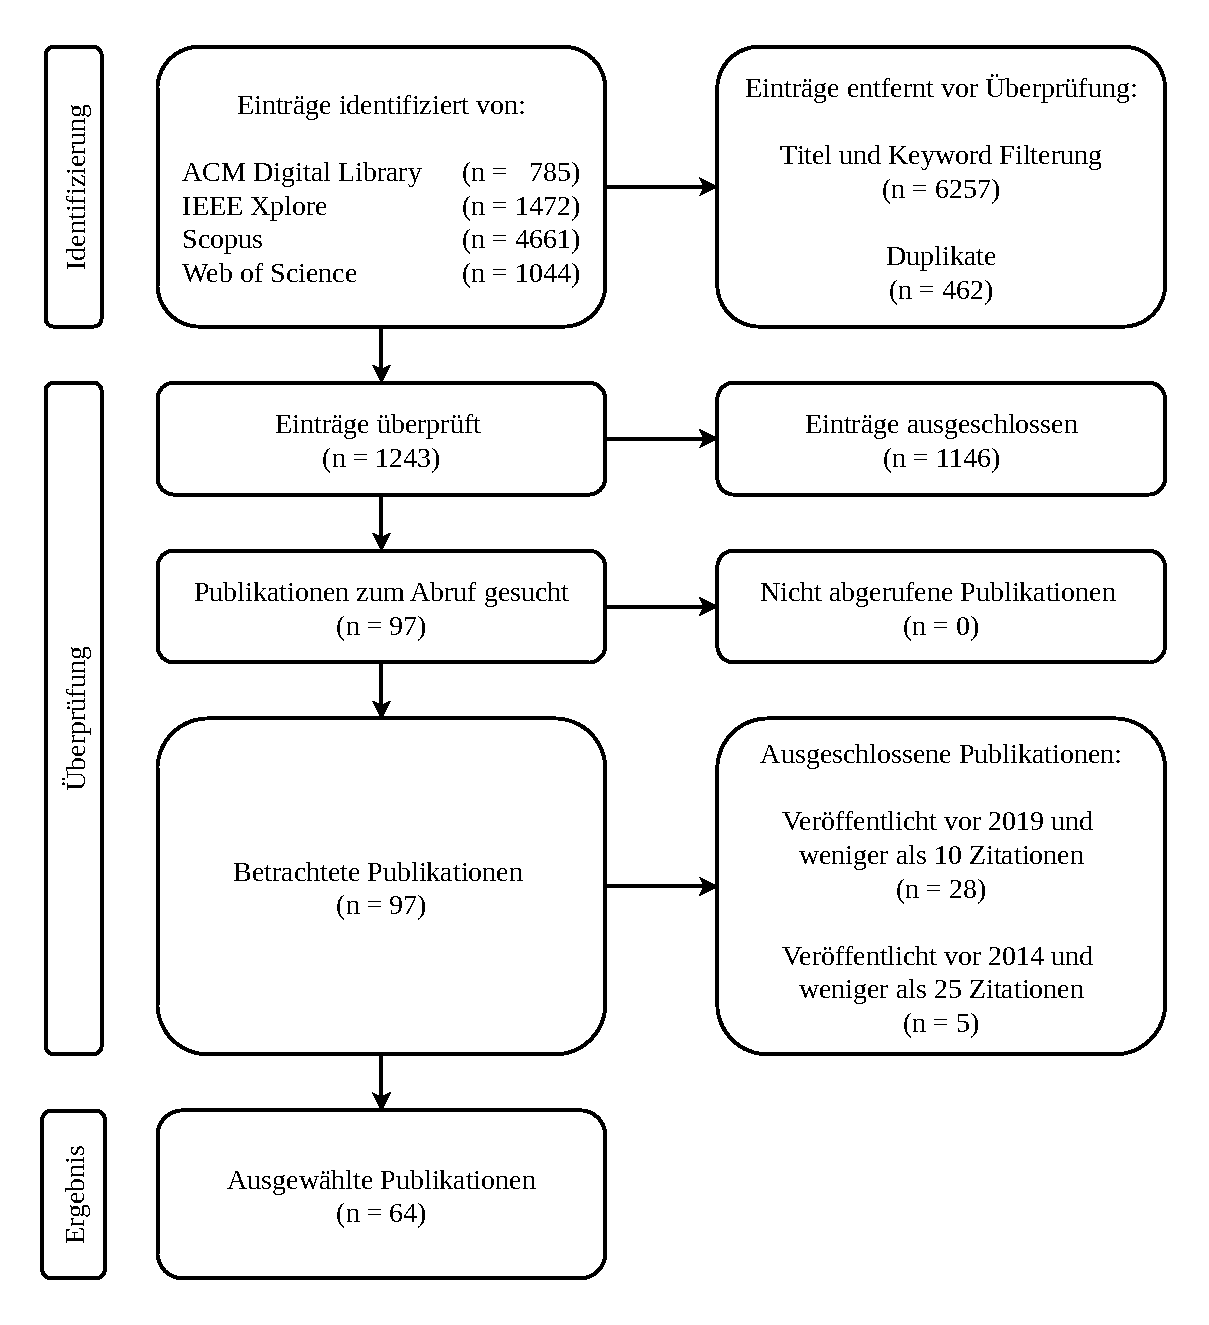
\includegraphics[width=\textwidth]{diagrams/PRISMA.pdf}
    \caption{PRISMA Diagramm}
    \label{figure:stand-der-technik:literaturrecherche:prisma-diagram}
\end{figure}

\subsection{Implementierungen}\label{section:stand-der-technik:literaturrecherche:implementierungen}

Es gibt eine Vielzahl an verschiedenen Implementierungen von online IDEs. Um einen Überblick über die unterschiedlichen Ansätze und die Änderungen über den Verlauf der Zeit zu bekommen, werden im Folgenden einige ausgewählte IDEs vorgestellt. Dabei werden die IDEs zeitlich sortiert vorgestellt.

\paragraph{Adinda}
Deursen et al. (2010) \cite{van_deursen_adinda_2010} beschreiben eine online IDE namens Adinda. Die grundlegende Idee von Adinda ist die Zerlegung der Funktionalität einer IDE in einen leichtgewichtigen Client sowie mehrere zusammenarbeitende (Web-)Services. Diese Services sollen dann bestimmte Aufgaben erfüllen, wie z.B. Kompilierung, Testen, kollaboratives Editieren und Datenerhebung. Es werden weiterhin verschiedenste Forschungsfragen aufgestellt, die für das vorgestellte System von Interesse sind. Die prototypische Implementierung von Adinda basiert auf WWWorkspace \cite{ryan_web_2007} und nutzt serverseitig die Eclipse IDE \cite{noauthor_eclipse_nodate}. Der Prototyp unterstützt das Erstellen von Nutzer-Workspaces, Java Projekten, Paketen und Klassendateien sowie Syntax Highlighting, Kompilierung und Code-Vervollständigung.

\paragraph{CEclipse}
Wu et al. (2011) \cite{wu_ceclipse_2011} stellen die online IDE Cloud Eclipse (CEclipse) vor. Die Ziele von CEclipse sind:
\begin{enumerate}
    \item die Bereitstellung von Funktionen der Eclipse IDE \cite{noauthor_eclipse_nodate}, wie zum Beispiel Code-Vervollständigung
    \item die Behandlung von den online IDE spezifischen Sicherheitsproblemen \quoted{\textit{Wrong file operations}}, \quoted{\textit{Banned operation calling}} und \quoted{\textit{Excessive resource consumption}}
    \item die Ausnutzung von Cloud Computing Möglichkeiten, um Entwickler besser zu unterstützen.
\end{enumerate}
Für $1.$ wurde ein entsprechendes Protokoll entwickelt, was es ermöglicht, die gewünschten Funktionen der Eclipse IDE aufzurufen und das Ergebnis im Browser darzustellen. Um die in $2.$ genannten Probleme handhaben zu können, wird ein \textit{Program Behavior Analysis Service} beschrieben. Durch die Einschränkung des Dateisystems auf einen speziellen Ordner kann das Problem \quoted{Wrong file operations} gelöst werden. Das Verbieten bzw. Erlauben von Methoden über eine Blacklist bzw. eine Whitelist kann zur Lösung des Problems \quoted{Banned operation calling} angewendet werden. Durch eine Zeitbegrenzung von laufenden Prozessen kann schließlich auch das Problem \quoted{Excessive resource consumption} behoben werden. Für $3.$ werden über den \textit{Program Behavior Mining Service} Daten über die Nutzung der IDE gesammelt werden. Diese Daten können dann z.B. dazu genutzt werden, dem Entwickler häufig verwendete Befehle mit höherer Priorität vorzuschlagen.

\paragraph{Collabode}
Goldman et al. (2011) \cite{goldman_real-time_2011} beschreiben Collabode, eine kollaborative online IDE für Java. Collabode ermöglicht es mehreren Nutzern gleichzeitig Änderungen an Dateien vorzunehmen. Die Änderungen werden in Echtzeit zwischen den Nutzern synchronisiert. Dabei wird ein spezieller Algorithmus verwendet. Dieser Algorithmus sorgt dafür, dass nur Änderungen eingepflegt werden, die keinen syntaktischen Fehler beinhalten oder erzeugen. Dadurch wird sichergestellt, dass Nutzer nur ihre eigenen Fehler sehen und das Programm unabhängig von den ggf. vorhandenen Fehlern ihrer Teammitglieder kompilieren können. Collabode nutzt EtherPad \cite{noauthor_etherpad_nodate} als Code Editor im Frontend und die Eclipse IDE \cite{noauthor_eclipse_nodate} für die Bereitstellung von Kompilierung, Syntax Highlighting, etc. im Backend.

\paragraph{CoRED}
Lautamäki et al. (2012) \cite{lautamaki_cored_2012} stellen den Collaborative Real-time Editor (CoRED) vor, einen online Code Editor für Java Programme. CoRED nutzt den ACE Editor \cite{noauthor_ace_nodate} im Frontend sowie das Java Development Kit (JDK) \cite{noauthor_jdk_nodate} zur Kompilierung im Backend. Fehlermeldungen während des Kompiliervorgangs werden an den Client zurückgesendet und dann im Frontend angezeigt. Zur Bereitstellung von Echtzeit Kollaboration wird der Algorithmus \textit{Differential Synchronization with shadows} \cite{fraser_differential_2009} von Neil Fraser eingesetzt. Weitere Features von CoRED sind das Sperren von Code Bereichen für andere Nutzer sowie die Möglichkeit, Kommentare im Code zu hinterlassen. Auf diese Kommentare können dann andere Nutzer antworten, wodurch eine weitere Interaktionsmöglichkeit besteht. Weiterhin bietet CoRED auch Code-Vervollständigung als Funktion an.

\paragraph{IDEOL}
Tran et al. (2013) \cite{tran_interactive_2013} stellen die online IDE IDEOL vor. IDEOL erlaubt es Nutzern, in Echtzeit miteinander zu kollaborieren. Dies beinhaltet das gleichzeitige Bearbeiten von Dateien mit Synchronisierung der Änderungen zwischen den Nutzern sowie ein Diskussionsforum mit einem Tagging-Mechanismus. Über diesen Mechanismus können Nutzer Codezeilen oder ganze Dateien in einer Diskussion taggen. Weiterhin können Nutzer auch Dateien an ihre Nachrichten anhängen. Zudem bietet IDEOL eine Übersicht über die Änderungen im Code. IDEOL bietet Support für die Entwicklung von C/C++ Programmen und erlaubt auch die Kompilierung, Ausführung sowie das Debuggen von diesen. Um die Echtzeit Kollaboration zu ermöglichen, unterscheidet IDEOL zwischen exklusiven und nicht-exklusiven Operationen. Zu den exklusiven Operationen zählen die Kompilierung, Ausführung und das Debuggen eines Programms. Dateien werden über einen Server synchronisiert und dort gespeichert. Die Behandlung von gleichzeitigen Operationen wird mithilfe eines Operational Transformation Algorithmus \cite{sun_operational_1998} vorgenommen. Exklusive Operationen werden auf der im Server persistent gespeicherten Version ausgeführt, sodass die im Arbeitsspeicher des Servers vorhandene Version weiterhin zur Bearbeitung verwendet werden kann. Nguyen et al. (2016) \cite{nguyen_enhancing_2016} nutzen IDEOL für die web-basierte kollaborative Umgebung EduCo. Das Ziel von EduCo ist die Bereitstellung von Funktionen für Lehrende und Lernende, besonders im Hinblick auf deren Interaktion und Kollaboration.

\paragraph{TouchDevelop}
Ball et al. (2015) \cite{ball_beyond_2015} beschreiben die online IDE TouchDevelop. Das Hauptfeature von TouchDevelop ist die Speicherung aller Programmänderungen, Versionen, Laufzeitinformationen, Bugs sowie Kommentare, Fragen und Feedback von Nutzern in einer zentralen Datenbank. Diese Daten können über entsprechende APIs abgefragt werden. Die Nutzeroberfläche von TouchDevelop unterscheidet sich stark von anderen textbasierten Editoren. So bekommt der Nutzer eine Auswahl an kontextabhängigen Optionen, z.B. if-Anweisungen, for-Schleifen oder verfügbare Variablen. Alle IDE Funktionen sind offline verfügbar, da sie komplett auf der Clientseite implementiert sind. Weiterhin nutzt TouchDevelop eine eigene Programmiersprache. Diese folgt dem imperativen Programmierparadigma, besitzt ein starkes Typsystem sowie eine Vielzahl an plattformübergreifenden APIs.

\paragraph{CodePilot}
Warner und Guo (2017) \cite{warner_codepilot_2017} stellen die online IDE CodePilot vor. Diese ermöglicht es Nutzern, Webapplikationen mithilfe von HTML, CSS und JavaScript zu entwickeln. Zudem können Nutzer mithilfe von Firepad \cite{noauthor_firepad_nodate} gleichzeitig an Projekten arbeiten. Weiterhin bietet CodePilot eine GitHub \cite{noauthor_github_nodate} Integration, wodurch Nutzer ihre Projekte aus GitHub importieren können. Über diese Integration werden auch bei jedem Commit die entsprechenden Änderungen an GitHub zurückgesendet. Weiterhin können Nutzer über einen Aktivitätsfeed die aktuellen Ereignisse nachverfolgen und mithilfe eines integrierten Text-Chats miteinander kommunizieren. Durch den Ace-Editor \cite{noauthor_ace_nodate} werden außerdem Syntax Highlighting und Code-Vervollständigung bereitgestellt. Zusätzlich bietet CodePilot die Möglichkeit, Issues zu erstellen. Diese werden dann mit GitHub synchronisiert und es wird ein Snapshot des aktuellen Projekts auf GitHub hinterlegt. Bei der Erstellung von Issues können auch Screenshots angefügt werden. Jede Issue enthält die Referenz auf den entsprechenden Snapshot des Projekts.

\paragraph{RIDE}
Über mehrere Publikationen hinweg wird die Entwicklung der Reflex IDE (RIDE) beschrieben. Zunächst wird von Bastrykina et al. (2021) \cite{bastrykina_developing_2021} ein entsprechender Kernel mit dem Xtext Framework \cite{noauthor_xtext_nodate} entwickelt. Dieser kann in der Eclipse IDE verwendet werden, um Funktionen wie Code-Vervollständigung und Code-Generation für die domainspezifische Sprache Reflex verfügbar zu machen. Zudem wird auch eine Integration mit dem \ac{LSP} \cite{noauthor_language-server-protocol_nodate} erreicht, wodurch diese Features auch für andere Code Editoren nutzbar sind. Darauf aufbauend wird von Gornev und Liakh (2021) \cite{gornev_ride_2021} die Konzipierung und Implementierung einer auf Theia basierten Web-Variante von RIDE vorgestellt. Gornev et al. (2022) \cite{gornev_towards_2022} beschreiben ein System, welches Docker verwendet, um die Web-Version von RIDE für mehrere simultane Nutzer bereitstellen zu können. Gornev und Bondarchuk (2023) \cite{gornev_towards_2023} stellen ein Framework vor, welches Echtzeit-Kollaboration in RIDE ermöglicht. Kuznetsov und Zyubin (2024) \cite{kuznetsov_development_2024} beschreiben darüber hinaus die Entwicklung eines Projektmanagement-Systems für RIDE.

\paragraph{PyodideU}
Jefferson et al. (2024) \cite{jefferson_pyodideu_2024} beschreiben eine IDE, die es Nutzern ermöglicht Python Code im Browser zu schreiben und auszuführen. Dabei wird das Programm des Nutzers lokal in dessen Browser durchgeführt. Dies wird durch den Einsatz von PyodideU, einer erweiterten Version der auf WebAssembly basierenden Python Distribution Pyodide \cite{noauthor_pyodide_nodate}, erreicht. Zusätzlich wird den Nutzern auch eine Grafikbibliothek samt eines Debuggers angeboten, der es ermöglicht, Zeile für Zeile und auch rückwärts durch das Programm zu gehen und die entsprechenden Änderungen an der Grafik zu sehen. Weiterhin wird durch PyodideU auch die synchrone Eingabe von Daten unterstützt, während Python im Main-Thread des Browsers läuft. Zudem wird auch ein Dateisystem bereitgestellt. Insgesamt wurde die IDE sowohl von Studenten als auch von Lehrenden als hilfreich wahrgenommen.

\paragraph{CS50}
Malan (2024) \cite{malan_containerizing_2024} beschreibt die verschiedenen Ansätze zur Bereitstellung einer integrierten Entwicklungsumgebung für die Teilnehmer des Einführungskurses in die Programmierung (CS50) an der Harvard University. Zunächst wurde seit 2007 ein On-Campus Cluster für die Studenten angeboten. Studenten konnten sich über SSH mit diesem verbinden und dort ihre Programme ausführen. Dieser Cluster wurde 2008 mithilfe von Amazon Web Services (AWS) \cite{noauthor_amazon_nodate} in die Cloud überführt. Diese cloud-basierte Lösung wurde 2011 durch Client-seitige virtuelle Maschinen ersetzt. In 2015 wurde eine auf Docker basierende Lösung erarbeitet, die zunächst die Cloud9 IDE \cite{noauthor_aws-cloud9_nodate} als Frontend nutzte. In 2021 wurde schließlich eine auf Github Codespaces aufbauende Lösung eingeführt, die \ac{VSCode} \cite{noauthor_vscode_nodate} als Code Editor verwendet.
\subsection{Architekturmuster}\label{section:stand-der-technik:literaturrecherche:architekturmuster}

Die betrachteten Publikationen beschreiben eine Vielzahl an verschiedenen online IDEs. Dabei kann eine Unterteilung in die folgenden drei Kategorien erfolgen:

\begin{itemize}
      \item \textbf{Client-Server-basierte Lösungen} \\
            Systeme dieser Art zeichnen sich dadurch aus, dass sie eine Client-Server-Archi-tektur verwenden. Hierbei werden Features, die nicht innerhalb eines Browsers ausgeführt werden können (z.B. Kompilierung) über einen entsprechenden Server bereitgestellt. Beispiele für derartige online IDEs sind u.a. Adinda \cite{van_deursen_adinda_2010}, CEclipse \cite{wu_ceclipse_2011} und Collabode \cite{goldman_real-time_2011}.
      \item \textbf{Browser-basierte Lösungen} \\
            Systeme dieser Art zeichnen sich dadurch aus, dass alle Features im Browser des Nutzers ausgeführt werden können, ohne die Hilfe eines separaten Servers. Beispiele für derartige online IDEs sind u.a. TouchDevelop \cite{ball_beyond_2015} und auf PyodideU aufbauende IDE \cite{jefferson_pyodideu_2024}.
      \item \textbf{Cloud-basierte Lösungen} \\
            Systeme dieser Art zeichnen sich dadurch aus, dass sie als Cloud-Service angeboten werden können. Meist erhalten Nutzer eine komplett eigene Umgebung samt Dateisystem, Compiler, Debugger und weiteren Tools. Diese Lösungen nutzen oftmals Containerisierung. Beispiele für derartige online IDEs sind u.a. AWS Cloud9 \cite{noauthor_aws-cloud9_nodate} und GitHub Codespaces \cite{noauthor_github-codespaces_2024}.
\end{itemize}
\subsection{Vorteile}\label{section:stand-der-technik:literaturrecherche:vorteile}

Online IDEs bieten eine Vielzahl an Vorteilen gegenüber lokalen IDEs. Diese Vorteile werden im Folgenden erläutert.

\paragraph{Keine Installation}
Ein Vorteil von online IDEs ist die Tatsache, dass diese keine Installation benötigen \cite{srinivasa_bad_2022}\cite{tran_interactive_2013}\cite{yang_evaluations_2018}. Somit wird es Nutzern ermöglicht direkt mit der Programmierung zu beginnen ohne zuvor die benötigte Software auf ihrem System installieren zu müssen. Dadurch ist es auch möglich die IDE auf Systemen auszuführen, auf denen sie sonst nicht installierbar wäre, wie z.B. mobile Endgeräte \cite{jefferson_pyodideu_2024}\cite{ball_beyond_2015}\cite{uehara_javascript_2019}. Im Bezug auf die Lehre erlaubt es den Lehrenden und Lernenden sich besser auf die Inhalte der Lehrveranstaltung zu konzentrieren, da sie weniger Zeit damit verbringen müssen systemabhängige Probleme mit der Einrichtung der IDE zu lösen \cite{valez_student_2020}.

\paragraph{Zeit- und Ortsunabhängigkeit}
Nutzer können jederzeit und von überall auf online IDEs zugreifen, solange sie einen entsprechenden Browser sowie eine Internetverbindung haben. Weiterhin können einige komplett im Browser nutzbare IDEs nach dem erstmaligen Laden auch offline genutzt werden \cite{jefferson_pyodideu_2024}. Außerdem erlaubt eine serverseitige Speicherung von Daten einen systemunabhängigen Zugriff auf diese \cite{ball_beyond_2015}. Somit können Nutzer selbst wählen, wann und mit welchem Gerät sie die IDE nutzen möchten, ohne von Zugriffszeiten und spezieller Hardware abhängig zu sein.

\paragraph{Einheitliche Umgebung}
Nutzern kann, unabhängig von ihrem System, eine einhaltliche Entwicklungsumgebung angeboten werden \cite{molnar_evaluation_2023}\cite{tran_interactive_2013}. Somit können systemabhängige bzw. versionsabhängige Probleme vermieden werden, was z.B. in der Lehre dazu führt, dass Lehrende und Lernende weniger Zeit für die Behebung derartiger Probleme aufbringen müssen \cite{valez_student_2020}. Außerdem können Client-Server sowie cloudbasierte online IDEs die Benutzererfahrung für Nutzer mit weniger performanten Systemen verbessern, da ein Teil der Berechnungen von einem externen Server durchgeführt wird.

\paragraph{Einbindbarkeit in Lernmanagementsysteme}
Ein weiterer Vorteil von online IDEs ist die vereinfachte Einbindbarkeit von online IDEs in \ac{LMS}, wie z.B. Moodle \cite{noauthor_moodle_nodate}. Da online IDEs im Browser des Nutzers ausgeführt werden können diese direkt in LMS eingebunden werden. Weiterhin können durch die Implementierung entsprechender Schnittstellen, wie z.B. \ac{LTI} \cite{noauthor_lti_nodate}, auch weitere Funktionen ermöglicht werden, wie z.B. die automatische Bewertung der Lösungen von Lernenden. Diese Art der Integration kann die Benutzererfahrung der Lernenden verbessern.

\paragraph{Einfachere Datenerhebung}
Online IDEs können die Erhebung von Nutzerdaten vereinfachen \cite{efopoulos_wipe_2005}\cite{singh_pyguru_nodate}\cite{helminen_recording_2013}. So können u.a. Cursorbewegungen, Code-Änderungen und Zeitaufwand aufgenommen und später analysiert werden. Mithilfe der Nutzerdaten können z.B. Lehrende erkennen bei welchen Aufgaben Studenten die meisten Probleme haben bzw. womit sie die meiste Zeit verbringen.

\paragraph{Skalierbarkeit}
Browser- sowie cloudbasierte IDEs besitzen eine hohe Skalierbarkeit. Browserbasierte IDEs können nachdem sie im Browser des Nutzers geladen wurden ohne bzw. mit geringen zusätzlichen Serverressourcen genutzt werden \cite{ball_beyond_2015}\cite{jefferson_pyodideu_2024}. Cloudbasierte IDEs können sich an dynamische Lastverhältnisse anpassen \cite{noauthor_azure-cloud-services_nodate}\cite{noauthor_ec2-autoscaling_nodate}. So kann für jeden Nutzer beim Starten der IDE eine entsprechende Instanz gestartet werden, die beim Verlassen der IDE wieder gestoppt wird. Dabei ist der Cloud-Anbieter für die Bereitstellung der entsprechenden Serverressourcen verantwortlich. Klassische Client-Server Implementierungen können auch die Skalierbarkeit erhöhen, wenn man die zuvor genannten Vorteile betrachtet.
\subsection{Nachteile}\label{section:stand-der-technik:literaturrecherche:nachteile}

Neben den zuvor beschriebenen Vorteilen besitzen online IDEs auch einige Nachteile, welche im Folgenden beschrieben werden.

\paragraph{Onlinezwang}
Ein Nachteil von online IDEs ist der oftmals damit verbundene Onlinezwang und die damit einhergehenden Probleme, die durch Latenzen, Instabilitäten und Ausfälle des Netzwerks ausgelöst werden \cite{kats_software_2012}\cite{leisner_good-bye_2019}. So können Latenzen zu einer schlechteren Nutzererfahrung führen, indem z.B. während einer Echtzeit Kollaboration die Änderungen anderer Nutzer stark verzögert ankommen. Instabilitäten können dazu führen, dass Änderungen verloren gehen bzw. der Nutzer auf eine stabilere Verbindung warten muss. Netwerkausfälle bedeuten in vielen Fällen, dass der Nutzer nicht mit der Programmierung fortfahren kann bis die Netzwerkverbindung wiederhergestellt wird. Außerdem kann es auch vorkommen, dass ein Fehler auf der Serverseite auftritt, wodurch Nutzer die online IDE nicht nutzen können. In diesem Fall müssen Nutzer darauf warten, bis das zugrunde liegende Problem behoben wird.

\paragraph{Abhängigkeit von Anbietern}
In den meisten Fällen besitzen Nutzer keine Kontrolle über die installierte Software \cite{kats_software_2012}. Sollte der Anbieter Updates durchführen kann dies dazu führen, dass zuvor funktionierende Programme des Nutzers nun versionsabhängige Fehler beinhalten. Weiterhin können die angebotenen IDEs auch komplett eingestellt werden, wodurch Nutzer keine Möglichkeit mehr besitzen diese zu nutzen. Zudem können Anbieter auch ihre Preise anpassen, wodurch die Kosten für die online IDE steigen können.

\paragraph{Implementierungs und Verwaltungsaufwand}
Der Implementierungs- und Verwaltungsaufwand von online IDEs kann sehr hoch sein \cite{malan_standardizing_2022} und somit einige der Vorteile von online IDEs aufwiegen. In gewissen Szenarien ist auch die Skalierbarkeit von online IDEs ein Problem, da diese oftmals mit erhöhten Kosten oder einem entsprechend höherem Verwaltungsaufwand verbunden ist. Diese Probleme sind entsprechend gravierender, wenn kein entsprechendes Personal für verfügbar ist und diese Aufgaben z.B. an Lehrende übertragen werden.

\paragraph{Sicherheit}
Anbieter von online IDEs müssen sicherstellen, dass Nutzer keine ungewünschen Aktionen ausführen können, die das System beeinträchtigen könnten. Derartige Aktionen sind z.B. \quoted{Wrong file operations}, \quoted{Banned operation calling}, \quoted{Excessive resource consumption} \cite{wu_ceclipse_2011} und \quoted{Arbitrary code execution} \cite{srinivasa_bad_2022}.

\paragraph{Erweiterbarkeit}
Zudem sind viele der während der Literaturrecherche gefundenen online IDEs sehr anwendungsspezifisch und somit in einigen Aspekten stark eingeschränkt, z.B. in den unterstützten Editoren, Programmiersprachen sowie den vorhandenen Einstellungs- und Erweiterungsmöglichkeiten. Weiterhin werden viele der gefundenen IDEs nicht mehr angeboten bzw. unterstützt und oftmals sind diese auch nicht quelloffen.


\subsection{Anforderungen}\label{section:stand-der-technik:literaturrecherche:anforderungen}

% Anforderungen:
% \begin{itemize}
%     \item Angemessenes Nutzerinterface
%     \item Syntax-Highlighting
%     \item Code-Vervollständigung
%     \item Kompilierung
%     \item Debugging
%     \item Kollaboration
%     \item (Erweiterbarkeit)
%     \item Sehr anwendungsspezifisch (z.B. Flashing von Microcontrollern, Rollenwechsel in Kollaboration)
%     \item Kommunikationsmöglichkeiten
%     \item Projektmanagement Features
%     \item Versionskontrolle
%     \item Programmiersprachen Support
%     \item Programmausührung
%     \item Testen
%     \item Input / Output
%     \item Guides für Nutzer
%     \item Möglichkeiten zur Datenerhebung
%     \item Interfaces für Lehrende
% \end{itemize}

Anforderungen an online IDEs sind meist sehr anwendungsspezifisch. Dementsprechend ist ein für die Zielgruppe angemessenes Nutzerinterface von hoher Bedeutung. Ein Student, der bereits mehrere Programmierkurse belegt hat und Erfahrungen mit IDEs sammeln konnte wird ein ihm vertrautes Interface mit bereits bekannten Funktionen wertschätzen, während das gleiche Interface einen Schüler, der gerade erst anfängt Programmieren zu lernen, überfordern würde. Ein für Schüler ausgelegtes Interface würde umgekehrt den Studenten frustrieren, da dieser ggf. bereits bekannte Funktionen nicht nutzen kann. Im Allgemeinen sollten aber die in einer IDE verwendeten Code Editoren Standardfunktionen wie z.B. Syntax Highlighting und Code-Vervollständigung für textbasierte Programmiersprachen unterstützen. Weiterhin sind oftmals auch die Kompilierung und Ausführung sowie das Debugging und Testen von Programmen wichtige Anforderungen an online IDEs. Zudem sollten den Nutzern auch Möglichkeiten zur Kollaboration angeboten werden. Dabei kann es den Nutzern unter anderem ermöglicht werden gleichzeitig an Projekten zu arbeiten, wobei gleichzeitig auch entsprechende Kommunikationsmöglichkeiten bereitgestellt werden können. Allerdings kann die Kollaboration auch asynchron über Versionskontrollsysteme wie z.B. Git \todoaddref[]{Git} und über Foren z.B. innerhalb eines verwendeten LMS ermöglicht werden. Eine weitere Anforderung ist die Möglichkeit zur Datenerhebung.